\section{Finite Element Neutron Diffusion}
\label{sec:neutronDiffusion}

\begin{frame}{Multigroup Neutron Diffusion Equation}
  In conventional notation, the multigroup neutron diffusion equation can be
  written.
  \begin{equation}
    \label{eq:multigroup_diffusion}
    - \grad \cdot ( D_g(\vr) \grad \phi_g(\vr)) + \Sigma_{r,g}(\vr) \phi_g(\vr)= 
      \frac{\widetilde{\chi_g}(\vr)}{\keff} 
      \sum_{g'=1}^{G} \nu\Sigma_{f,g'}(\vr) 
      \phi_{g'}(\vr) + \sum_{g'=1 \; g' \ne g}^{G} 
      \Sigma_{s,g' \rightarrow g}(\vr) \phi_{g'}(\vr)
  \end{equation}
  \begin{conditions} % custom environment designed for this purpose
    D_g(\vr)    & diffusion coefficient for energy group $g$ \units{cm}, \\
    \phi_g(\vr) & scalar neutron flux for energy group $g$
      \units{$\frac{1}{\text{cm}^2 \; \text{s}}$}, \\
    \Sigma_{r,g}(\vr) & macroscopic removal cross-section for energy group $g$ 
      \units{$\frac{1}{\text{cm}}$}, \\
    \widetilde{\chi_g}(\vr) & effective fission spectrum for energy group $g$,\\
    \keff & effective neutron multiplication factor, \\
    \nu \Sigma_{f,g}(\vr) & 
      \parbox[t]{\columnwidth}{number of fission neutrons times microscopic 
        fission \\
        cross-section in energy group $g$ \units{$\frac{1}{\text{cm}}$}, }\\
    \Sigma_{s,g' \rightarrow g} (\vr) & 
      \parbox[t]{\columnwidth}{macroscopic scatter cross-section from
      energy group $g'$ to\\
      energy group $g$ \units{$\frac{1}{\text{cm}}$},} \\
    G & total number of energy groups (typically $G=33$)%.
  \end{conditions}
\end{frame}

\begin{frame}{Boundary Conditions}
  Consider a domain $\Omega$ with boundary $\partial \Omega$ and let $\nhat$ be
  the outward-normal unit vector.
  \begin{enumerate}
    \item Mirror.
      \begin{equation}
        \grad \phi_g(\vr) \cdot \nhat = 0 \; \forall \; \vr \in \partial \Omega
      \end{equation}
    \item Albedo. 
      \begin{equation}
        D_g(\vr) \grad \phi_g(\vr) \cdot \nhat + \albedo \phi_g(\vr)
          = 0 \; \forall \; \vr \in \partial \Omega
      \end{equation}
    \item Zero Flux. 
      \begin{equation}
        \phi_g(\vr) = 0 \; \forall \; \vr \in \partial \Omega
      \end{equation}
  \end{enumerate}
\end{frame}

\begin{frame}{\gls{fem} Discretization}
  Divide the domain $\Omega$ into a set of unstructured finite elements 
  (e.g. Delaunay triangulation).
  \begin{gather}
    \label{eq:set_of_elements}
    \Omega = \Omega_1 \cup \Omega_2 \cup \Omega_3 \cup \ldots \cup
      \Omega_{N_E}  \\
    \Omega = \{\Omega_e\} \; \text{for} \; e = 1,2,\ldots,N_E \\
    \Omega_i \cap \Omega_j = \emptyset \; \text{for} \; i \ne j
  \end{gather}
  \begin{figure}
    \centering
    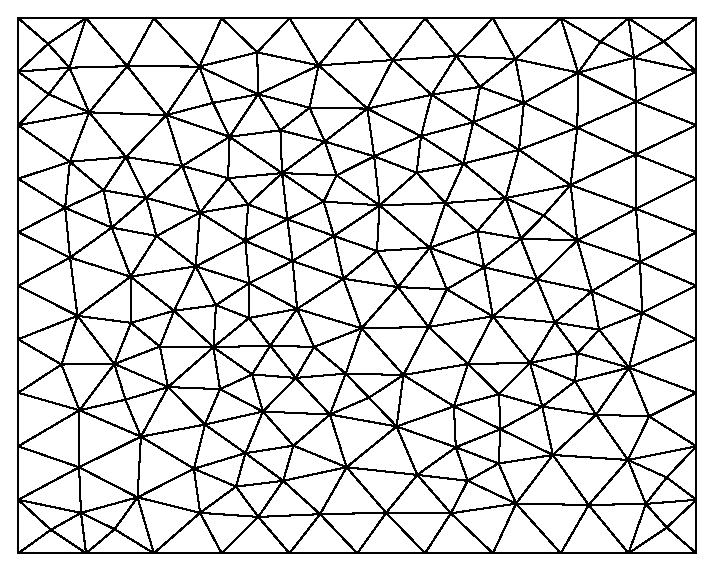
\includegraphics[width=0.4\textwidth]{./figs/fixed0}
    \caption{Example Square Mesh.}
    \label{fig:fixed0}
  \end{figure}
\end{frame}

\begin{frame}{Combining Neutron Source}
  \begin{itemize}
    \item Neutron sources are combined into a single term.
    \item This will resemble the \gls{fem} formulation.
  \end{itemize}
  \begin{equation}
    \label{eq:multigroup_source}
    - \grad \cdot( D_g(\vr) \grad \phi_g(\vr)) + \Sigma_{r,g}(\vr) \phi_g(\vr) = 
      q_g(\vr)
  \end{equation}
  \begin{align}
    q_g(\vr) &= q_{g,e} \; \forall \; \vr \in \Omega_e \\
    \phiavg_{g,e} &= \frac{1}{N_p} \sum_{i \in \Omega_e}^{N_p} \phi_{i,g}
  \end{align}

  \begin{itemize}
    \item Neutron source $q_g(\vr)$ is constant over an element $\Omega_e$.
    \item Cross-sections constant within an element.
  \end{itemize}
\end{frame}

\begin{frame}{\glsentryfull{fem}}
  Multiply the multigroup neutron diffusion equation by a testing function
  $v(\vr) \in H_1(\Omega)$ and integrate over the problem domain. $H_1(\Omega)$
  is a Sobolev space.
  
  \vspace{0.25in}
  This yields the \textbf{Weak Form} of the problem.
  \begin{align}
    \label{eq:fem_weak_form}
    - \int_{\Omega} \grad \cdot (D_g(\vr) \grad \phi_g(\vr)) v(\vr) \; d\vr
      + \int_{\Omega} \Sigma_{r,g}(\vr) \phi_g(\vr) v(\vr) \;d\vr &=
      \int_{\Omega} q_g(\vr) v(\vr) \;d\vr \\
    \label{eq:element_by_element}
    -\sum_{e=1}^{N_E} D_{g,e} 
      \int_{\Omega_e} \grad \cdot \grad \phi_g(\vr) v(\vr) \; d\vr +
      \sum_{e=1}^{N_E} \Sigma_{r,g,e} \int_{\Omega_e} \phi_g(\vr) v(\vr) 
      \;d\vr &= \sum_{e=1}^{N_E} q_{g,e} \int_{\Omega_e} v(\vr) 
      \; d\vr
  \end{align}
\end{frame}

\begin{frame}
  Use the Second Green's Theorem to rewrite the first integral
  \cite{textbookli}.
  \begin{multline} 
    -\sum_{e=1}^{N_E} D_{g,e} \int_{\partial \Omega_e} v(\vr) \grad
    \phi_g(\vr) \cdot \nhat \;ds + \sum_{e=1}^{N_E} 
      D_{g,e} \int_{\Omega_e} \grad \phi_g(\vr) \cdot \grad v(\vr) 
      \; d\vr + \\
      \sum_{e=1}^{N_E} \Sigma_{r,g,e} \int_{\Omega_e} \phi_g(\vr) v(\vr) 
     \; d\vr =
      \sum_{e=1}^{N_E} q_{g,e} \int_{\Omega_e} v(\vr) \; d\vr
  \end{multline}
\end{frame}

\begin{frame}{Galerkin Finite Element Method}
  Galerkin Finite Element Method assumes the solution $\phi_g(\vr)$ is a linear
  combination of chosen basis functions $\{\basis_i\}$.
  \begin{equation} 
    \label{eq:linear_combination}
    \phi_g(\vr) = \sum_{i=1}^{DOF} \upsilon_{g,i} \, \basis_i(\vr)
  \end{equation}
  Coefficients $\{\upsilon_{g,i}\}$ will be solved in a linear system.
  $v(\vr)$ is arbitrary such that $v(\vr) \in H_1(\Omega)$ and is chosen to be a
  linear combination of the basis functions with unit magnitude.
  \begin{equation} 
    \label{eq:linear_superposition}
    v(\vr) = \sum_{j=1}^{DOF} \basis_j(\vr)
  \end{equation}
\end{frame}

\begin{frame}{Linear System of Equations}
  Including albedo form of boundary condition and assumption of linear
  combination of basis functions.
  \begin{multline}
    \label{eq:linear_equation}
    \sum_{i=1}^{DOF} \upsilon_{i,g} \sum_{j=1}^{DOF} \left(
      \sum_{e=1}^{N_E} \albedo \int_{\partial \Omega_e}
      \basis_i(\vr)  \basis_j(\vr) \;ds +
      \sum_{e=1}^{N_E} D_{g,e} 
      \int_{\Omega_e} \grad \basis_i(\vr) \cdot \grad \basis_j(\vr)\;d\vr
      \right.
      + \\
      \left.
      \sum_{e=1}^{N_E} \Sigma_{r,g,e}
      \int_{\Omega_e} \basis_i(\vr) \basis_j(\vr) \; d\vr \right) =
      \sum_{i=1}^{DOF} \left(
      \sum_{e=1}^{N_E} q_{g,e} 
      \int_{\Omega_e} \basis_i(\vr) \; d\vr \right)
  \end{multline}

  Rewriting in the form common to \gls{fem}.
  \begin{equation}
    \label{eq:fem_notation}
    a_g(\basis_i,\basis_j) = f_g(\basis_i)
  \end{equation}
  In the form common to linear systems.
  \begin{gather}
    \label{eq:matrix_notation}
    \ma_g \, \vu_g = \vf_g \\
    \vu_g = \{\upsilon_{i,g}\}
  \end{gather}
\end{frame}

\begin{frame}{Properties of $\ma_g \, \vu_g = \vf_g$}
  Properties of the linear system include:
  \begin{itemize}
    \item Sparse.
    \item Matrix, $\ma_g$, is \gls{spd} \cite{textbookhughes}.
    \item Solution, $\vu_g$, is unique and bounded by Lax-Milgram Lemma 
      \cite{textbookli}.
  \end{itemize}
  Solution via \gls{cg} method 
  \cite{Kelley1995IterativeEquations}.

  It is natural to populate the matrix $\ma_g$ in an element-by-element 
  procedure.
  \begin{align}
    \label{eq:matrix_population}
    A_{i,j,g,e} &= \albedo \int_{\partial \Omega_e} \basis_i(\vr) 
      \basis_j(\vr) \; ds + D_{g,e} 
      \int_{\Omega_e} \grad \basis_i(\vr) \cdot \grad \basis_j(\vr) \;
      d\Omega_e \\
    &\qquad + \Sigma_{r,g,e} \int_{\Omega_e} \basis_i(\vr) \basis_j(\vr)
      \; d\Omega_e, \\
    \label{eq:vector_population}
    f_{i,g,e} &= q_{g,e} \int_{\Omega_e} \basis_i(\vr) \;d\Omega_e.
  \end{align}
  \begin{align}
    A_{i,j,g} &= \sum_{e=1}^{N_E} A_{i,j,g,e} \\
    f_{i,g} &=  \sum_{e=1}^{N_E} f_{i,g,e}
  \end{align}
\end{frame}

\begin{frame}{Integration}
  Integrals of interest:
  \begin{align}
    &\int_{\Omega_e} \grad \basis_i(\vr) \cdot \grad \basis_j(\vr) 
      \;d\vr \\
    &\int_{\Omega_e} \basis_i(\vr) \basis_j(\vr) \;d\vr \\
    &\int_{\Omega_e} \basis_i(\vr) \;d\vr \\
    &\int_{\partial \Omega_e} \basis_i(\vr) \basis_j(\vr) \;ds &
  \end{align}

  Options for integration:
  \begin{itemize}
    \item Analytic.
    \item Numeric (quadrature).
    \begin{itemize}
      \item Linear (Gaussian).
      \item Triangular.
    \end{itemize}
  \end{itemize}
\end{frame}

\begin{frame}{Triangular Elements}
  \begin{figure}
    \centering
    \subfloat[General Triangle Element.]
      {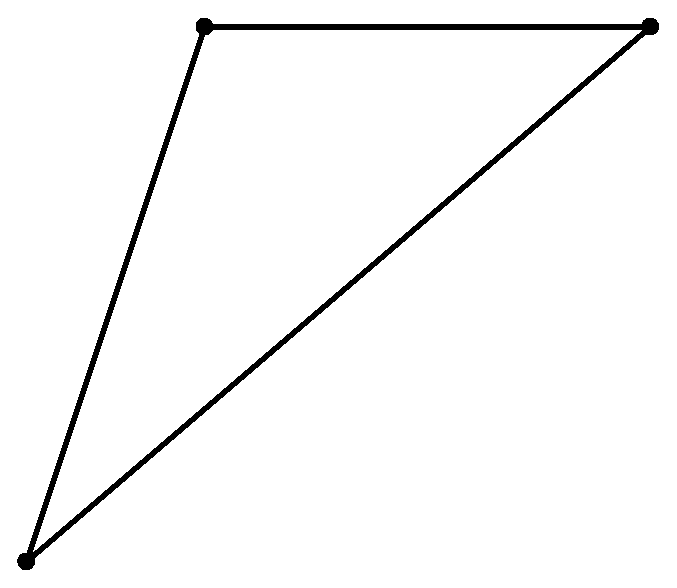
\includegraphics[width=0.35\textwidth]{sketch_triangle}}
    \vspace{0.2in}
    \subfloat[Reference Triangle.]
      {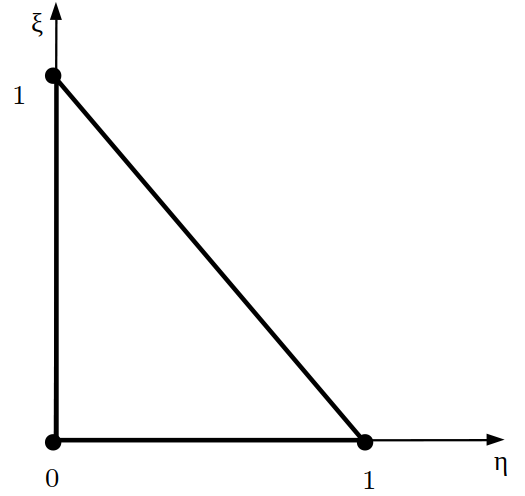
\includegraphics[width=0.35\textwidth]{Tref}}
    %\caption{Description of Triangle Elements.}
    \label{fig:triangle_elements}
  \end{figure}
\end{frame}

\begin{frame}{Wedge Elements}
  \begin{columns}
    \begin{column}{0.5\textwidth}
      \vspace*{\fill}
      \begin{figure}
        \centering
        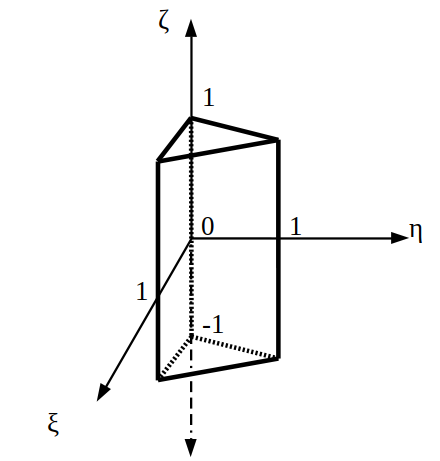
\includegraphics[width=0.8\textwidth]{Wref}
        \caption{Description of Reference Wedge.}
        \label{fig:Wref}
      \end{figure}
      \vspace*{\fill}
    \end{column}
    \begin{column}{0.5\textwidth}
      \begin{figure}
        \centering
        \subfloat[General Wedge Element.]
          {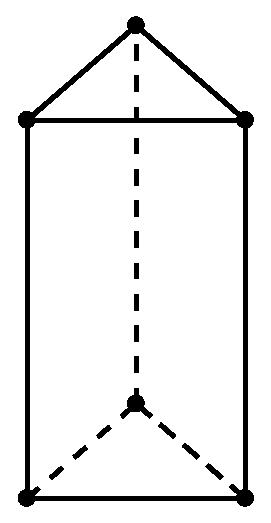
\includegraphics[width=0.4\textwidth]{wedge_sketch}}
        \hspace{0.1\textwidth}
        \subfloat[Distorted Wedge Element.]
          {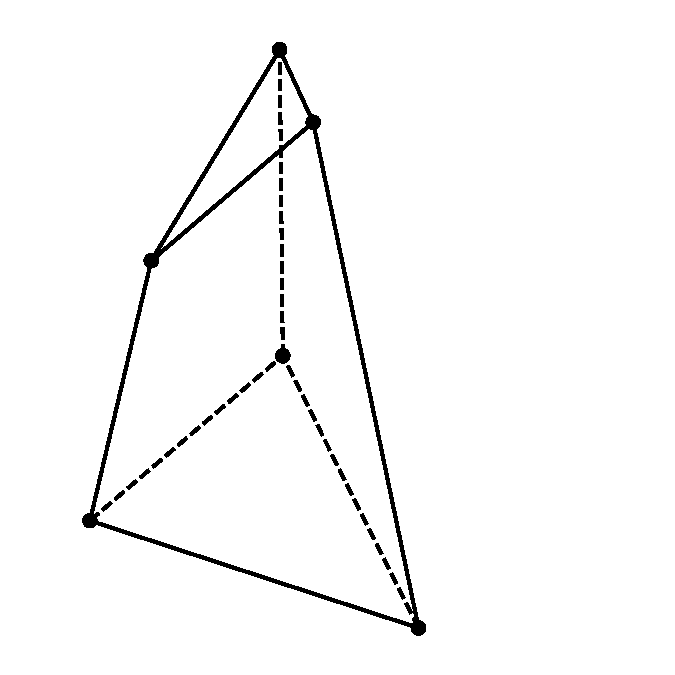
\includegraphics[width=0.4\textwidth]{wedge_stretch}}
        %\caption{Description of Wedge Elements.}
        \label{fig:sketch_wedge}
      \end{figure}
    \end{column}
  \end{columns}
\end{frame}

\begin{frame}{Matrix Ordering}
  \begin{itemize}
    \item Matrix is reordered to increase computational efficiency and compute
      the same solution.
    \item Nodes are re-indexed such that physically proximate nodes have
      proximate indices.
    \item Improve cache hits.
    \item \gls{rcm} order is chosen \cite{rcm}.
  \end{itemize}
  \vspace{-0.25in}
  \begin{figure}
    \centering
    \subfloat{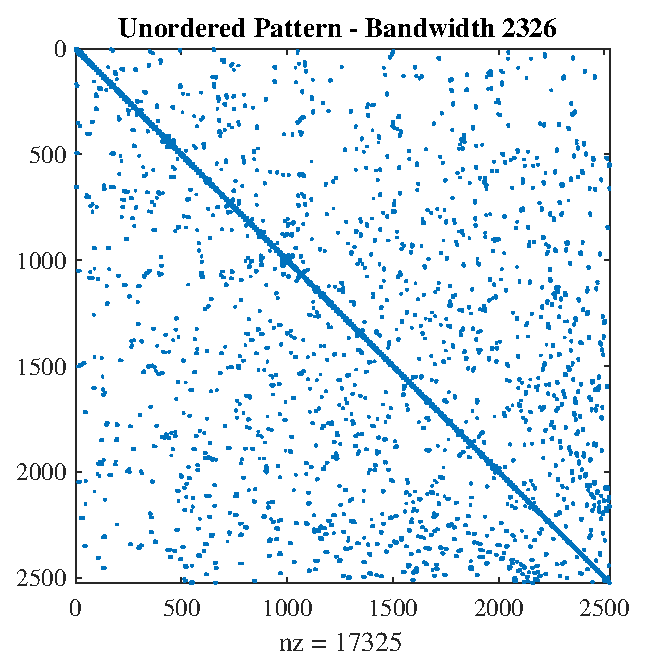
\includegraphics[width=0.4\textwidth]{uno_pattern}}
    \hspace{0.1in}
    \subfloat{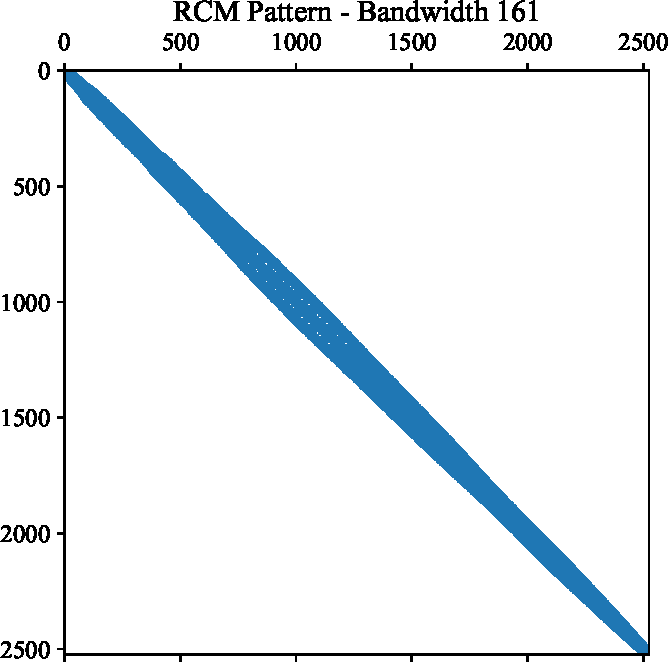
\includegraphics[width=0.4\textwidth]{rcm_pattern}}
    \label{fig:sparsity_pattern}
  \end{figure}
\end{frame}

\begin{frame}{Power Iteration Algorithm}

    \begin{algorithm}[H]
      \caption{\scriptsize General Iteration Scheme}
      \label{algorithm:general}
      \begin{algorithmic}[1]
      \State Read mesh from VTK.
      \State Initialize $\phiavg^{(0)}$.
      \State Order the nodes of the mesh into \gls{rcm} order.
        \label{state:rcm}
      \State Calculate $\Sigma_{s,g'\rightarrow g}$, $\Sigma_{r,g}$, and 
        $\nu \Sigma_{f,g}$ for each element.
      \State Calculate finite element matrix $\ma_g$ for each group. Store this. 
        \label{state:fem_matrix}
      \While{Power Iteration}
        \State Update the iteration counter. $s=s+1$
        \State Update $q_{fiss,g}$ and $q_{up,g}$ for all groups from previous 
          data $\phiavg^{(s-1)}$.
        \State Update $\widetilde{\chi_g}$ in each element using previous data.
          \label{state:chi_collapse}
        \For{$g=1,G$}
          \State Update $q_{down,g}$ from current data $\phiavg_g^{(s)}$
          \State Calculate total source in each element.
          \State Update finite element Vector $\vf_g$ with new source.
            \label{state:fem_vector}
          \State Solve $\ma_g \vu_g = \vf_g$ using an iterative technique
            (\gls{cg}).
          \State Parse $\vu_g$ for $\phi_g$ solution on nodes.
          \State Calculate element-average $\phiavg_g$.
        \EndFor
        \State Update $\keff$.
        \State Check convergence.
        \State Perform non-linear update if necessary and update $\ma_g$. 
          \label{state:nonlinear}
      \EndWhile
      \end{algorithmic}
    \end{algorithm}

\end{frame}
